% --
% machine learning

\section{Neural Networks for KWS}
\sectionheader{Neural Networks for KWS}

\begin{frame}
  \frametitle{Fully Connected Layer}
  \begin{columns}
    \begin{column}{0.45\textwidth}
      \begin{itemize}
        \item Output with activation $h$:
        \begin{equation*}
          \footnotesize
          \begin{aligned}
            \bm{z} = h(W \bm{x} + \bm{b})
          \end{aligned}
        \end{equation*}
        {\scriptsize with $\bm{x} \in \R^n$, $\bm{z} \in \R^m$, $\bm{b} \in \R^m$.}
        \vspace{0.2cm}
        \item Amount of Params:
        \begin{equation*}
          \footnotesize
          \begin{aligned}
            m \cdot n + m
          \end{aligned}
        \end{equation*}
        \item Amount of Operations:
        \begin{equation*}
          \footnotesize
          \begin{aligned}
            \mathcal{T}(W \bm{x} + \bm{b}) \approx 2 (m \cdot n) + m
          \end{aligned}
        \end{equation*}     
      \end{itemize}
    \end{column}
    \begin{column}{0.55\textwidth}
      \vspace{0.75cm}
      \centering
      \begin{figure} 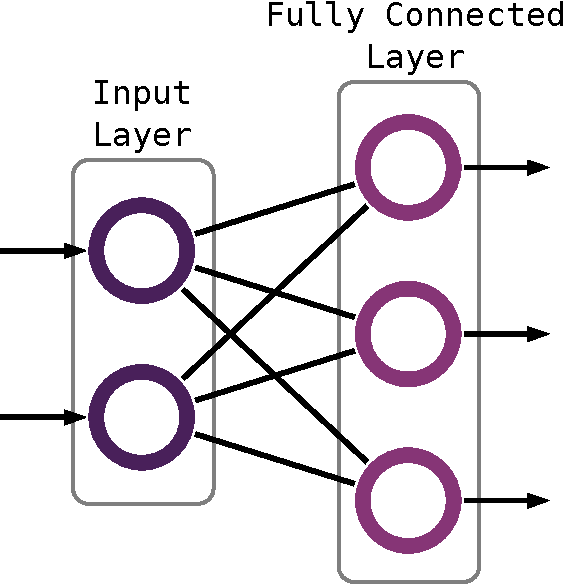
\includegraphics[width=0.55\textwidth]{../4_nn/figs/nn_theory_fc.pdf} \end{figure}
      \vfill
    \end{column}
  \end{columns}
\end{frame}

\begin{frame}
  \frametitle{Convolutional Layer}
  \begin{columns}
    \begin{column}{0.5\textwidth}
      \begin{itemize}
        \item j-th output channel $o_j$:
        \begin{equation*}
          \footnotesize
          o_j = \sum_{i} k_{i, j} \ast x_i,
        \end{equation*}
        \footnotesize
        with $x_i$ as i-th input channel and $k_{i, j}$ as kernel.   
      \end{itemize}
    \end{column}
    \begin{column}{0.5\textwidth}
      \centering
      \begin{figure} 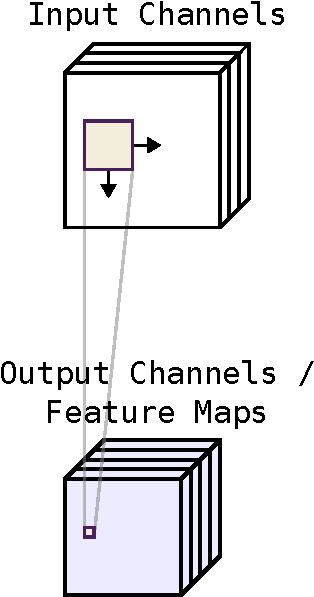
\includegraphics[width=0.45\textwidth]{./figs/nn_theory_cnn_scheme.pdf} \end{figure}
      \vfill
    \end{column}
  \end{columns}
\end{frame}

\begin{frame}
  \frametitle{Convolutional Layer Example}
  \begin{figure} 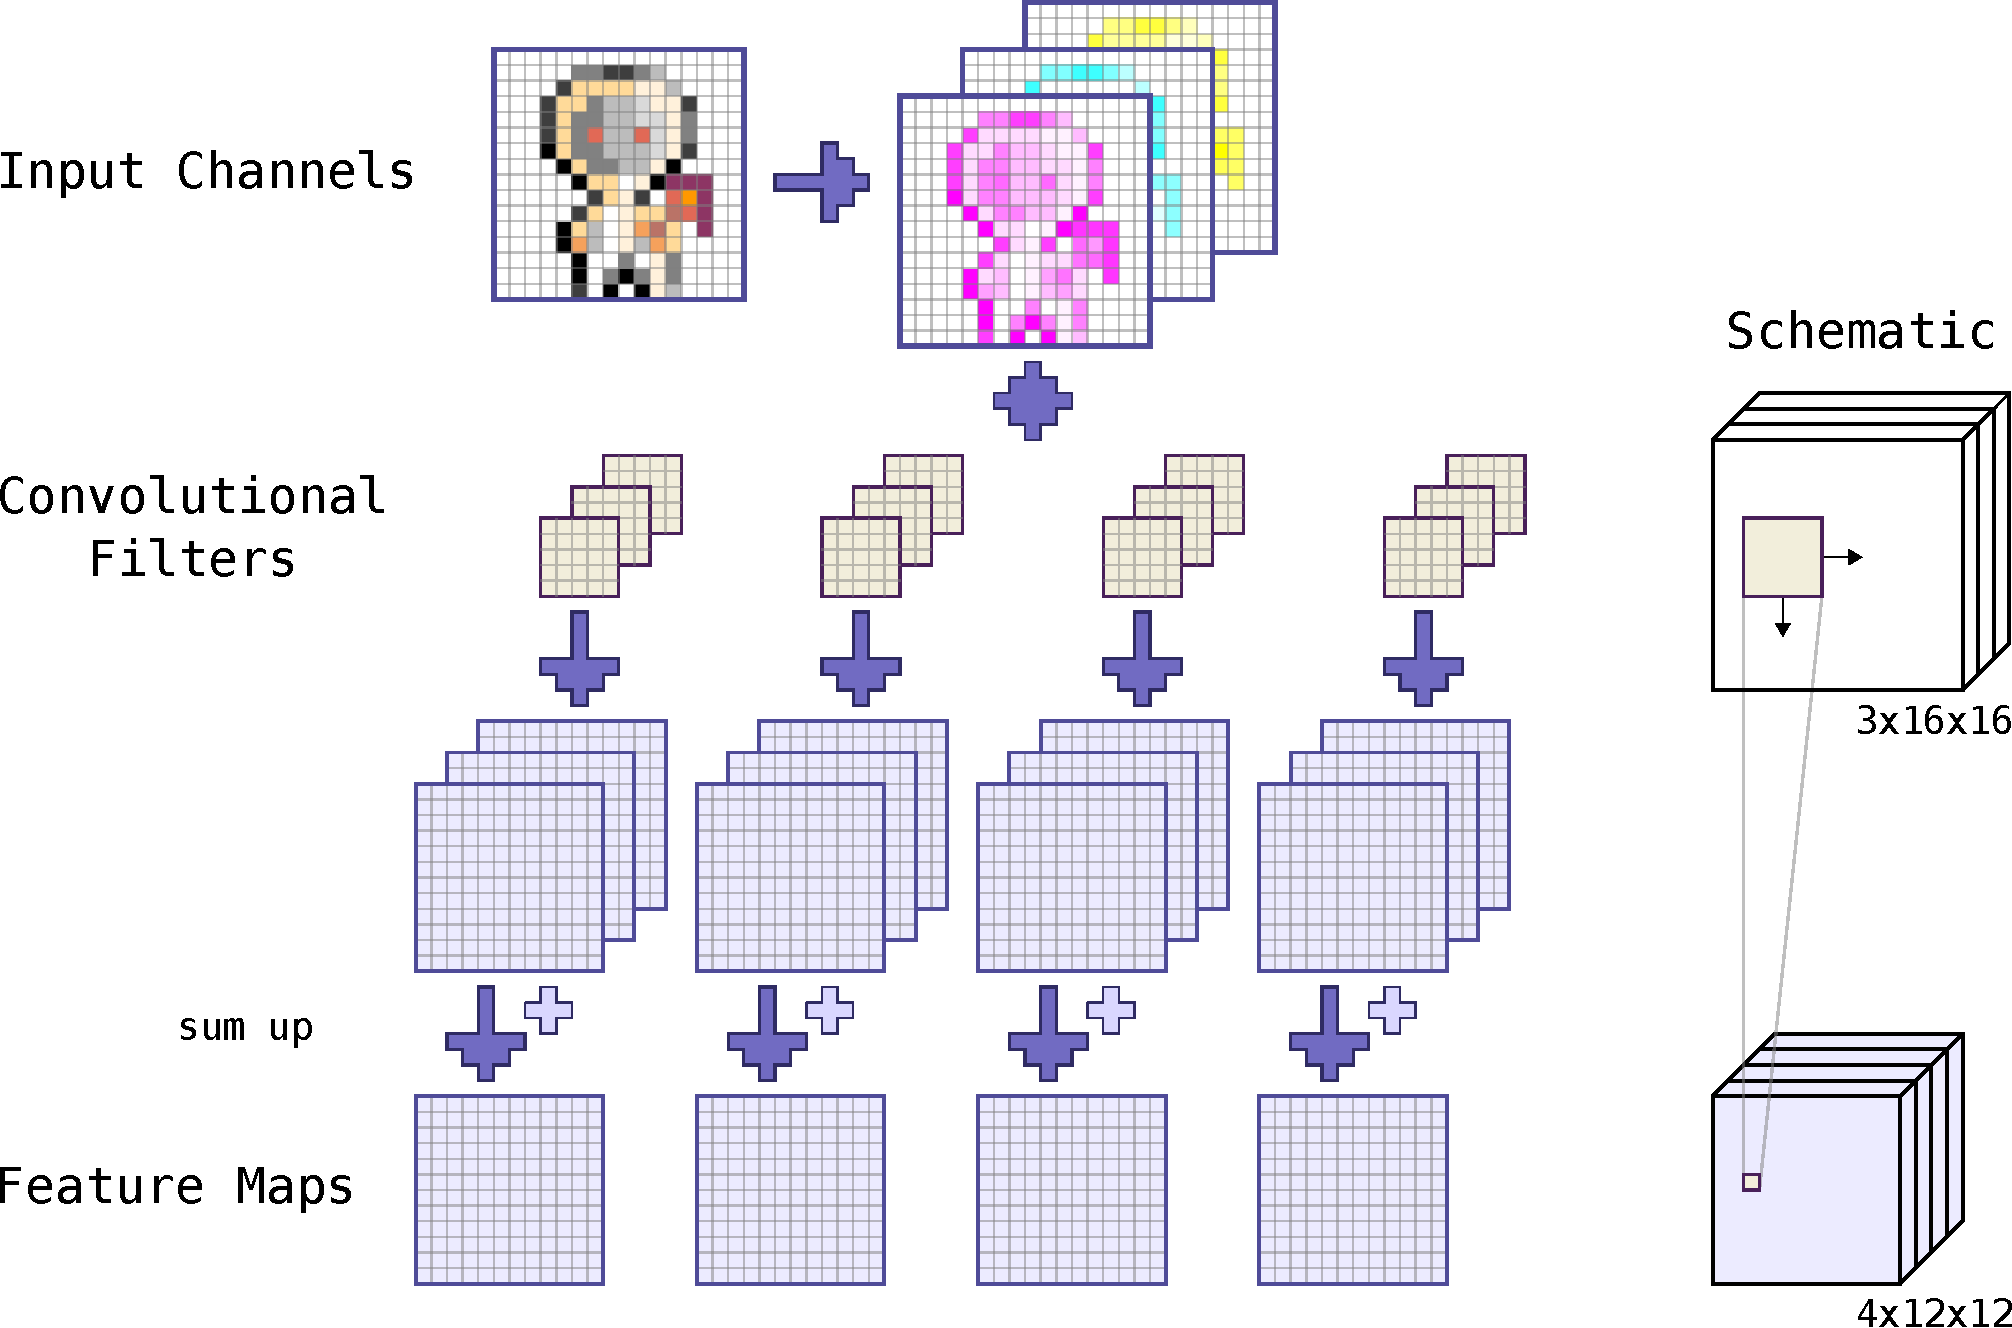
\includegraphics[width=0.8\textwidth]{../4_nn/figs/nn_theory_cnn_basics.pdf} \end{figure}
\end{frame}

\begin{frame}
  \frametitle{Traditional Network (conv-trad)}
  \begin{itemize}
    \item Layer Structure: Conv.: 2 + 1 max. pool, FC: 3 
    \item Num. Params: \textbf{\num{68396}}
    \item Num. Operations: \textbf{\SI{3770.98}{\kilo\ops}}
  \end{itemize}
  \begin{figure} 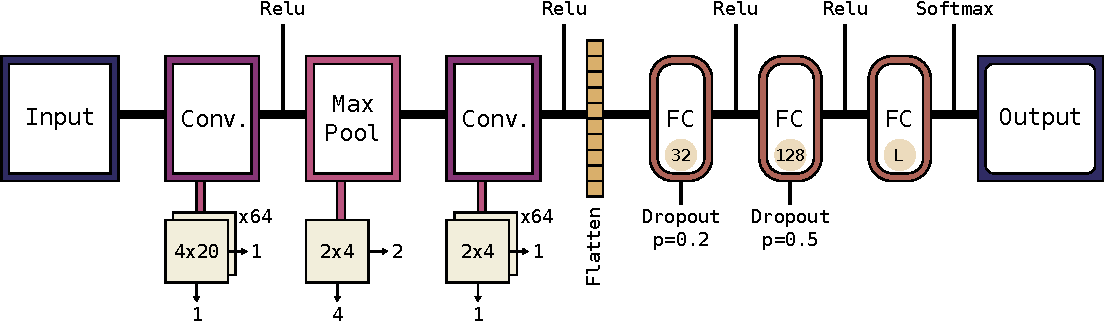
\includegraphics[height=0.35\textheight]{../4_nn/figs/nn_arch_cnn_trad.pdf} \end{figure}
\end{frame}

\begin{frame}
  \frametitle{Frequency Striding Network (conv-fstride)}
  \begin{itemize}
    \item Layer Structure: Conv.: 1, FC: 4
    \item Num. Params: \textbf{\num{47426}} 
    \item Num. Operations: \textbf{\SI{137.75}{\kilo\ops}}
  \end{itemize}
  \begin{figure} 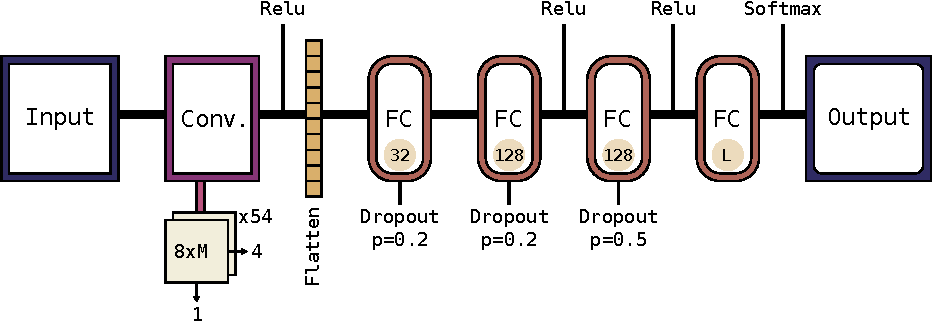
\includegraphics[height=0.35\textheight]{../4_nn/figs/nn_arch_cnn_fstride.pdf} \end{figure}
\end{frame}

\begin{frame}
  \frametitle{Time Striding Network(conv-jim)}
  \begin{itemize}
    \item Layer Structure: Conv.: 2, FC: 3
    \item Num. Params: \textbf{\num{29804}}
    \item Num. Operations: \textbf{\SI{862.40}{\kilo\ops}}
  \end{itemize}
  \begin{figure} 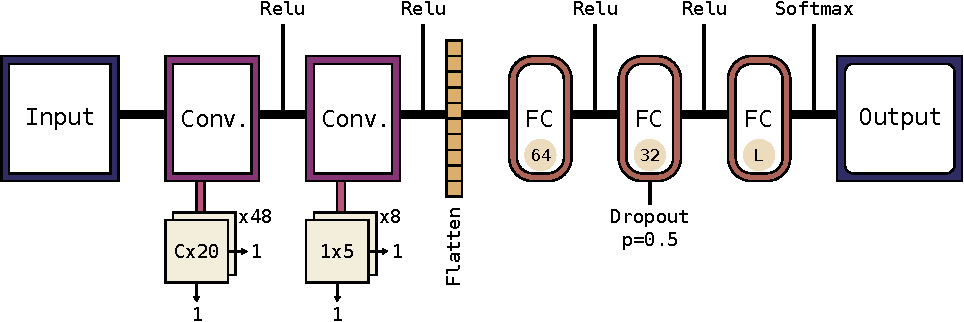
\includegraphics[height=0.35\textheight]{../4_nn/figs/nn_arch_cnn_jim.pdf} \end{figure}
\end{frame}


\begin{frame}
  \frametitle{GANs}
  \begin{itemize}
    \item consist of two adversarial networks:
    \begin{itemize}
      \footnotesize
      \item Discriminator (D) for binary classification of fake / real input
      \item Generator (G) to create image from the training dataset
    \end{itemize}
    \item Min-Max Solution for the Game between G and D:
  \end{itemize}
  \begin{equation*}
    \footnotesize
    \begin{aligned}
      \underset{G}{\min} \, \underset{D}{\max} \, V(D, G) = & \E_{\bm{x} \sim p_{data}(\bm{x})}\left[ \log D(\bm{x}) \right] + \\
      & \E_{\bm{z} \sim p_{\bm{z}}(\bm{z})}\left[ \log (1 - D(G(\bm{z}))) \right],
    \end{aligned}
  \end{equation*}
\end{frame}


\begin{frame}
  \frametitle{Adversarial Label Training}
  \begin{itemize}
    \item Version of conv-jim:
  \end{itemize}
  \begin{figure} 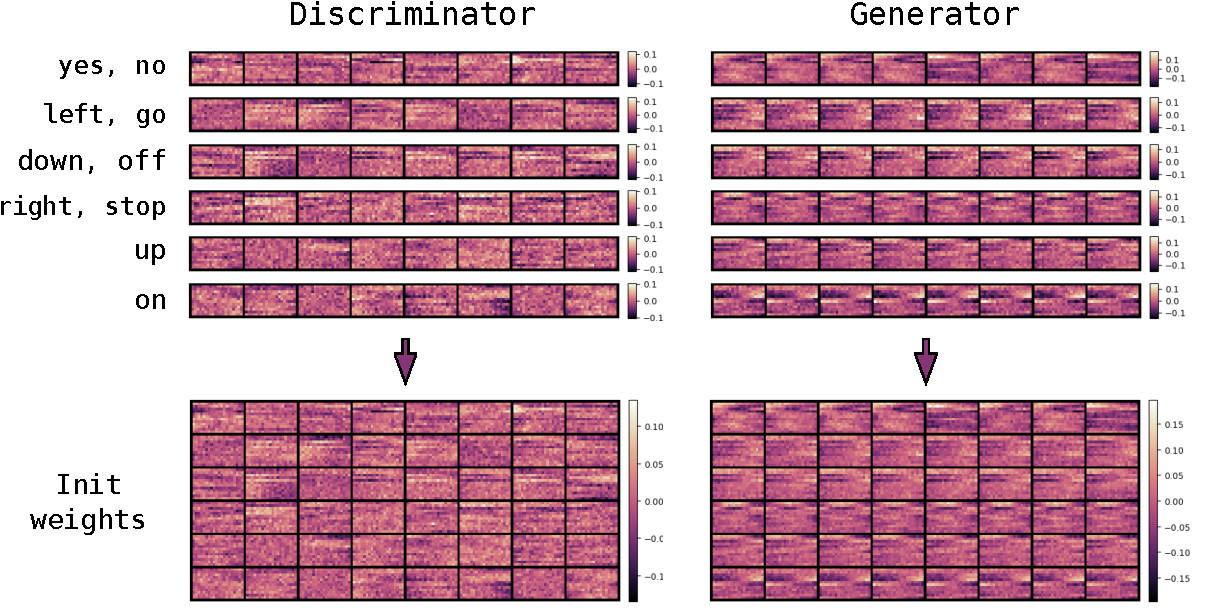
\includegraphics[height=0.5\textheight]{../4_nn/figs/nn_adv_label_scheme.pdf} \end{figure}
\end{frame}


\begin{frame}
  \frametitle{Wavenet Residual block}
  \begin{itemize}
    \item Residual block
  \end{itemize}
  \begin{figure} 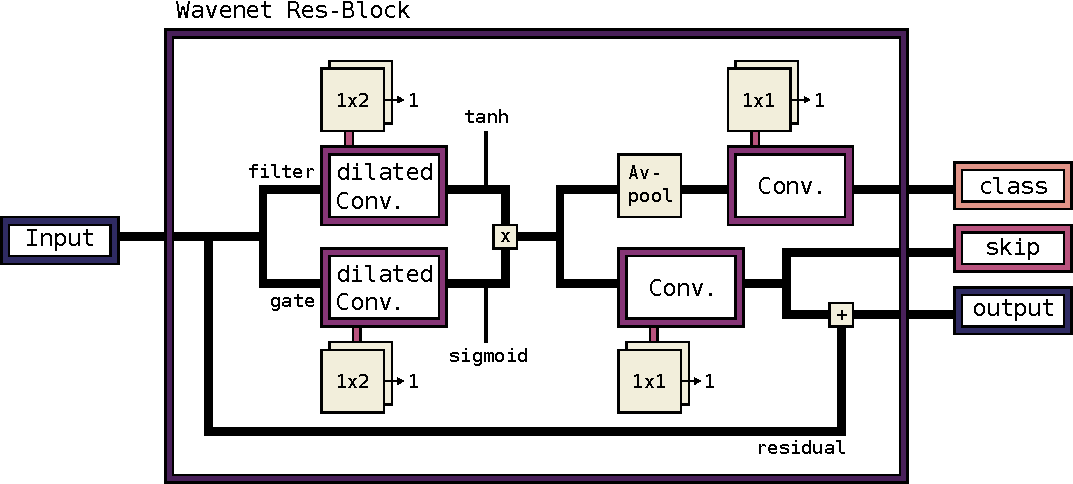
\includegraphics[height=0.45\textheight]{../4_nn/figs/nn_arch_wavenet_block.pdf} \end{figure}
\end{frame}

\begin{frame}
  \frametitle{Wavenet Architecture}
  \begin{itemize}
    \item Num. Params: \textbf{\num{33509}}
    \item Num. Operations: \textbf{\SI{36695.02}{\kilo\ops}}
  \end{itemize}
  \begin{figure} 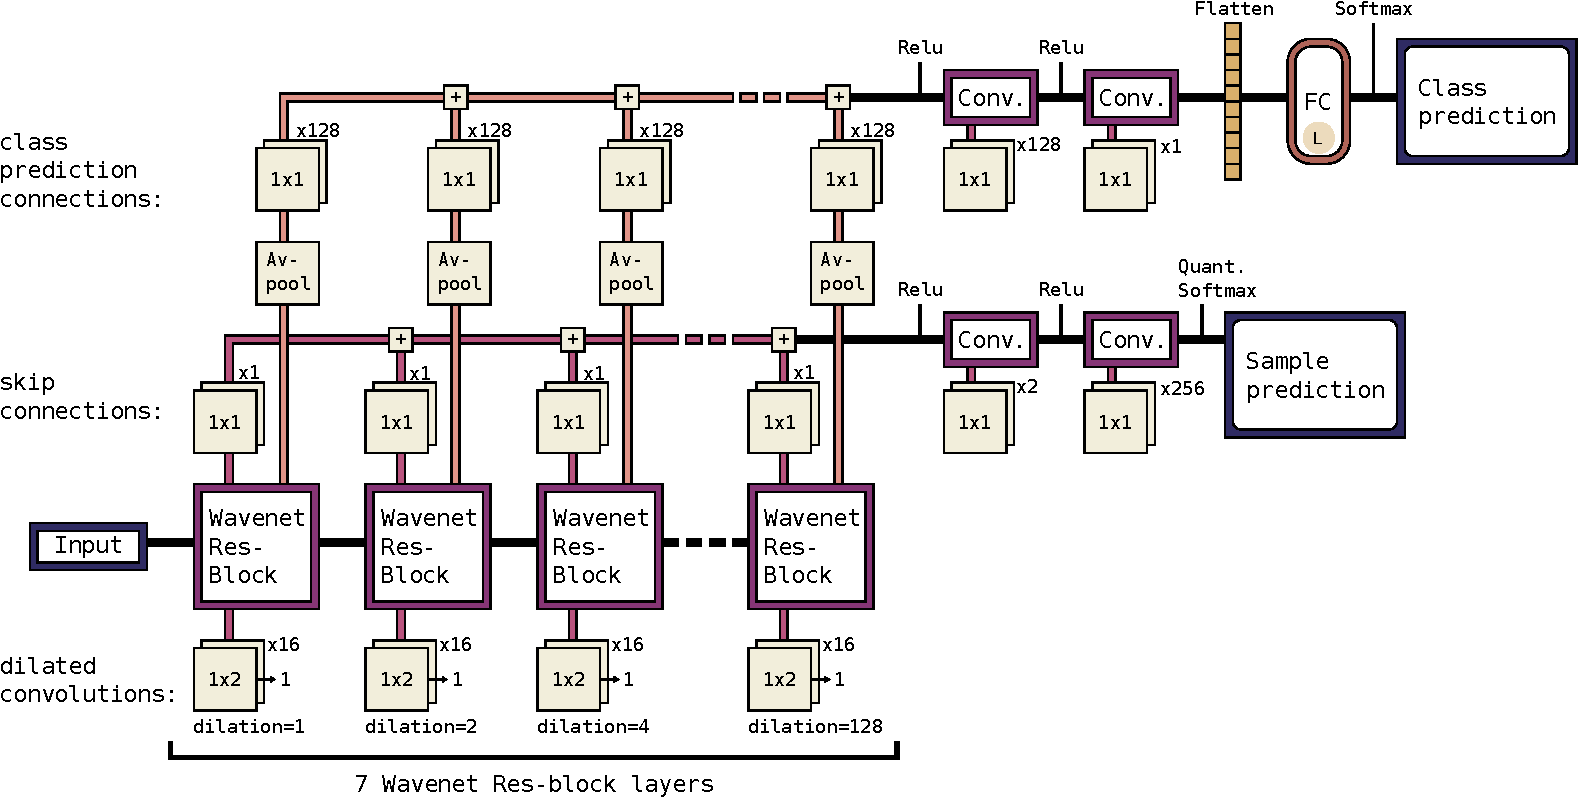
\includegraphics[height=0.5\textheight]{../4_nn/figs/nn_arch_wavenet_all.pdf} \end{figure}
\end{frame}